\ifnum\pdfoutput=0
  \def\pgfsysdriver{pgfsys-dvisvgm.def}
\fi
\documentclass[tikz,border=0pt]{standalone}
\usepackage{tikz}
\usetikzlibrary{arrows.meta}
\usepackage[scaled=0.92]{helvet}
\renewcommand{\familydefault}{\sfdefault}

% Colors matching blog _variables.scss and tree-shuffling header palette
\definecolor{bg}{HTML}{1E1E1E}
\definecolor{treeline}{HTML}{BEBEBE}
\definecolor{mutedline}{HTML}{555555}
\definecolor{mutedbox}{HTML}{6E6E6E}
\definecolor{digitcolor}{HTML}{D9D9D9}
\definecolor{muteddigit}{HTML}{808080}
\definecolor{swapcyan}{HTML}{19D4FA}
\definecolor{boxbg}{HTML}{252526}

% Closed rectangle macros using -- cycle so dvisvgm emits single-M SVG paths
\newcommand{\drawrect}[5]{
    \draw[#1] (#2, #3) -- (#4, #3) -- (#4, #5) -- (#2, #5) -- cycle;
}
\newcommand{\filldrawrect}[5]{
    \filldraw[#1] (#2, #3) -- (#4, #3) -- (#4, #5) -- (#2, #5) -- cycle;
}

\begin{document}
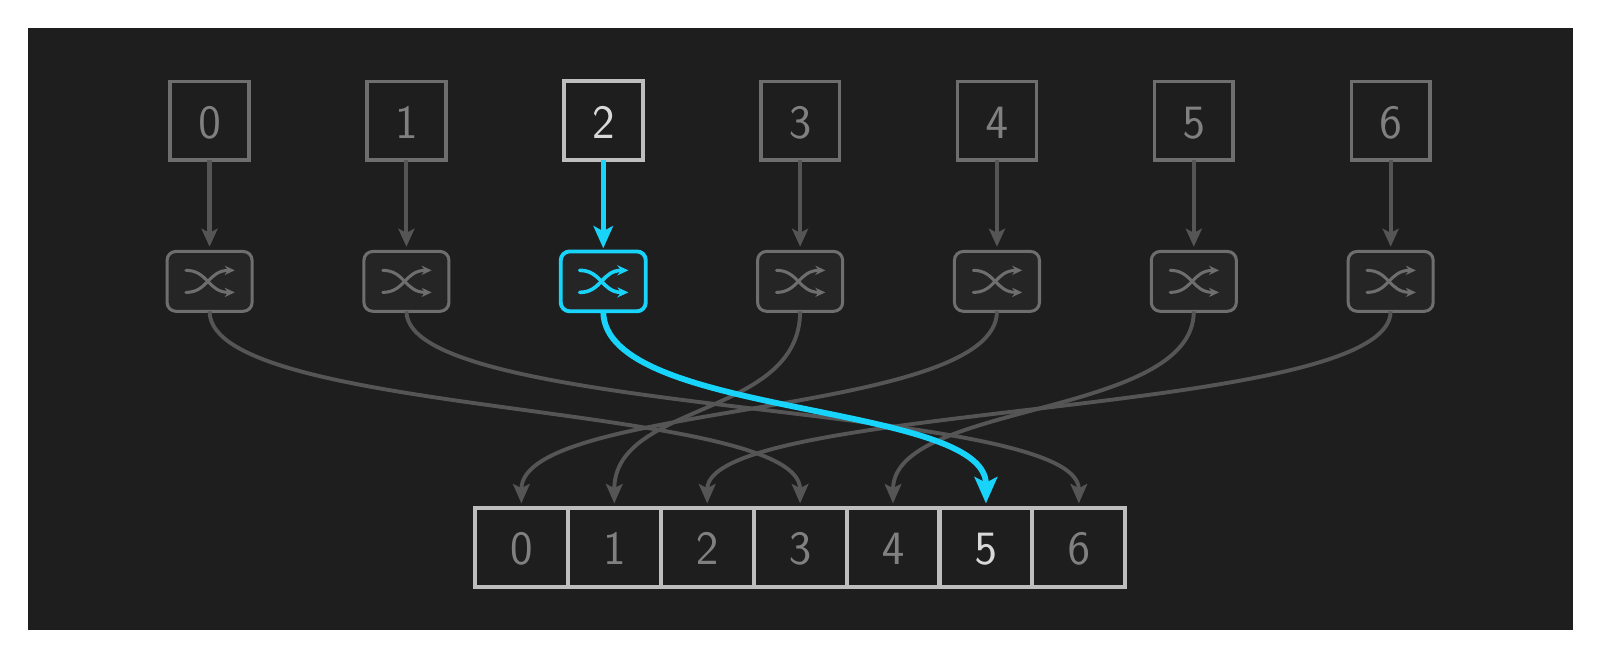
\begin{tikzpicture}[x=1cm, y=1cm]
    % Aspect ratio 2.5641 (matching 800 x 312), horizontal center at x = 9.16
    \path[use as bounding box] (-0.65, -1.55) rectangle (18.97, 6.102);
    \fill[bg] (-0.65, -1.55) rectangle (18.97, 6.102);

    % 7 elements (0..6) centered at x = 9.16
    \def\stepx{2.50}
    \def\topx{1.16}
    \def\arrw{1.18}
    \def\arrx{5.03}

    % Full 7-cycle bijection: 0->3, 1->6, 2->5 (cyan), 3->1, 4->0, 5->4, 6->2
    % 1. Muted background columns (0, 1, 3, 4, 5, 6)
    \foreach \i/\target in {0/3, 1/6, 3/1, 4/0, 5/4, 6/2} {
        \pgfmathsetmacro{\bx}{\topx + \i * \stepx}
        \pgfmathsetmacro{\sx}{\bx + 0.5}
        \pgfmathsetmacro{\tx}{\arrx + (\target + 0.5) * \arrw}

        % Separated input index box
        \drawrect{mutedbox, line width=1.3pt, line join=miter}{\bx}{4.42}{\bx + 1.0}{5.42}
        \node[color=muteddigit, font=\fontsize{19}{19}\selectfont, anchor=center]
            at (\sx, 4.90) {\i};

        % Vertical stem into isolated stateless permute node
        \draw[mutedline, line width=1.5pt, -{Stealth[length=6.5pt, width=5.8pt, inset=1.5pt]}]
            (\sx, 4.42) -- (\sx, 3.32);

        % Isolated stateless function box with shuffle icon
        \filldrawrect{mutedbox, fill=boxbg, line width=1.1pt, rounded corners=3.2pt}{\sx - 0.54}{2.50}{\sx + 0.54}{3.26}
        \draw[mutedbox, line width=1.1pt, line cap=round, -{Stealth[length=3.6pt, width=3.3pt]}]
            (\sx - 0.30, 3.02) .. controls (\sx - 0.02, 3.02) and (\sx - 0.02, 2.74) .. (\sx + 0.32, 2.74);
        \draw[mutedbox, line width=1.1pt, line cap=round, -{Stealth[length=3.6pt, width=3.3pt]}]
            (\sx - 0.30, 2.74) .. controls (\sx - 0.02, 2.74) and (\sx - 0.02, 3.02) .. (\sx + 0.32, 3.02);

        % Bijection curve to target array slot
        \draw[mutedline, line width=1.4pt, -{Stealth[length=7pt, width=6pt, inset=1.5pt]}]
            (\sx, 2.50) .. controls (\sx, 1.15) and (\tx, 1.35) .. (\tx, 0.06);
    }

    % Target contiguous 7-element array at the bottom: y from -1.0 to 0.0
    \drawrect{treeline, line width=1.5pt, line join=miter}{\arrx}{-1.0}{\arrx + 7 * \arrw}{0.0}
    \foreach \i in {1,...,6} {
        \pgfmathsetmacro{\dx}{\arrx + \i * \arrw}
        \draw[treeline, line width=1.5pt] (\dx, -1.0) -- (\dx, 0.0);
    }
    % Non-highlighted target array digits (slots 0, 1, 2, 3, 4, 6)
    \foreach \i in {0, 1, 2, 3, 4, 6} {
        \pgfmathsetmacro{\cx}{\arrx + (\i + 0.5) * \arrw}
        \node[color=muteddigit, font=\fontsize{19}{19}\selectfont, anchor=center]
            at (\cx, -0.52) {\i};
    }
    % Highlighted target array digit (slot 5, hit by cyan query 2)
    \pgfmathsetmacro{\cxFive}{\arrx + 5.5 * \arrw}
    \node[color=digitcolor, font=\fontsize{19}{19}\selectfont, anchor=center]
        at (\cxFive, -0.52) {5};

    % 2. Highlighted independent query in bright cyan (column 2 -> slot 5)
    \pgfmathsetmacro{\bxTwo}{\topx + 2 * \stepx}
    \pgfmathsetmacro{\sxTwo}{\bxTwo + 0.5}
    \pgfmathsetmacro{\txFive}{\arrx + 5.5 * \arrw}

    % Highlighted input box
    \drawrect{treeline, line width=1.5pt, line join=miter}{\bxTwo}{4.42}{\bxTwo + 1.0}{5.42}
    \node[color=digitcolor, font=\fontsize{19}{19}\selectfont, anchor=center]
        at (\sxTwo, 4.90) {2};

    % Cyan vertical stem into isolated permute node
    \draw[swapcyan, line width=2.0pt, -{Stealth[length=8pt, width=7pt, inset=1.8pt]}]
        (\sxTwo, 4.42) -- (\sxTwo, 3.30);

    % Highlighted isolated function box
    \filldrawrect{swapcyan, fill=boxbg, line width=1.4pt, rounded corners=3.2pt}{\sxTwo - 0.54}{2.50}{\sxTwo + 0.54}{3.26}
    \draw[swapcyan, line width=1.3pt, line cap=round, -{Stealth[length=4pt, width=3.6pt]}]
        (\sxTwo - 0.30, 3.02) .. controls (\sxTwo - 0.02, 3.02) and (\sxTwo - 0.02, 2.74) .. (\sxTwo + 0.32, 2.74);
    \draw[swapcyan, line width=1.3pt, line cap=round, -{Stealth[length=4pt, width=3.6pt]}]
        (\sxTwo - 0.30, 2.74) .. controls (\sxTwo - 0.02, 2.74) and (\sxTwo - 0.02, 3.02) .. (\sxTwo + 0.32, 3.02);

    % Cyan curve to target array cell 5
    \draw[swapcyan, line width=2.1pt, -{Stealth[length=9.5pt, width=8.2pt, inset=2pt]}]
        (\sxTwo, 2.50) .. controls (\sxTwo, 1.15) and (\txFive, 1.35) .. (\txFive, 0.06);

\end{tikzpicture}
\end{document}
